\chapter[Typesetting a Book in \LaTeX2e Using the WSPC Book Style]{Typesetting a Book in \LaTeX2e\\ Using the WSPC Book Style\label{ch1}}

\section{Introduction}\label{sec1.1}
This article explains how to use World Scientific's ws-book9x6
Document Class written in \LaTeX2e. Authors who use this system
correctly should find that writing their books is comparatively
easy, since the output will be in a form directly suitable for
camera-ready copy. In addition, the book will be produced quicker,
automatically fitting the in-house style by default. The article
itself was typeset using \verb|ws-book9x6.cls|.
You can obtain these files from our web pages at:
\url{http://www.worldscientific.com/page/authors/book-stylefiles} and
\url{http://www.icpress.co.uk/authors/stylefiles.shtml#books}.

\section{Using Other Packages}\label{sec1.2}
The class file loads the packages {\tt amsmath, amsfonts, amssymb,
graphicx, rotating, makeidx} at startup.

Please try to limit your use of additional packages\index{packages}
as they frequently introduce incompatibilities. This problem is not
specific to the WSPC styles; it is a general \LaTeX{} problem. Check
this manual to see whether the required functionality is already
provided by the WSPC class file. If you do need third-party
packages, ensure that you send them along with the book. In general,
you should use standard \LaTeX{} commands as much as possible.

User-defined macros should be placed in the preamble of the chapter,
and not at any other place in the document. Definitions made using
the commands \verb|\newcommand,| \verb|\renewcommand,|
\verb|\newenvironment| or \verb|\renewenvironment| should be used
with great care. Restricted usage of such definitions is encouraged.
Large macro packages and definitions that are not used in the book
should be avoided. Do not change existing environments, commands and
other standard parts of \LaTeX.

\section{Input Used to Produce This Paper}
An example of a master file for a book with 3 chapters and an
appendix might be:
\begin{verbatim}
\documentclass{ws-book9x6}
\usepackage{ws-book-thm}
\usepackage{ws-book-har}

\title{My Book Title}

\makeindex

\begin{document}

\titlepages
\begin{dedication}
\large Dedication Page (optional)
\end{dedication}
\blankpage
\input preface.tex

\tableofcontents

\setcounter{page}{1}
\input chapter1.tex
\input chapter2.tex
\input chapter3.tex
\input appendix.tex

\bibliographystyle{ws-book-har}
\bibliography{ws-book-sample}
%\input bibliography.tex

\printindex
\end{document}
\end{verbatim}

\vfill

\eject

\section{Layout}
In order to facilitate our processing of your book, please give
easily identifiable structure to the various parts of the text by
making use of the usual \LaTeX{} commands or by your own commands
defined in the preamble, rather than by using explicit layout
commands, such as \verb|\hspace, \vspace, \large, \centering|, etc.
Also, do not redefine the page-layout parameters.

\section{Master File}
Chapters should be written in separate files rather than creating
one long file. The complete book should be run from a master
file\index{master file} which in turn calls all chapters or allows
chapters that can be processed selectively using the \verb|\input|
command. Instructions for the preparation of the book, including
notes on preparing text which comprises Parts; Chapters; Section
headings; Lists; Floats that include Tables and Figures;
Mathematics; and References are discussed in this chapter.

\section{Subdocuments}
\subsection{Parts}\index{subdocuments!parts}
The interior of a book usually comprises three major divisions: the
{\it front matter}; the {\it text}; and the {\it back matter}. The
three main divisions in turn, may comprise several parts. Each part
(or chapters in the part) may be written by a single author or by
several authors contributing to a volume. A part is then further
subdivided into chapters and sections. A part heading always occurs
on a right-hand, odd-numbered page (recto). It is mandatory to leave
the following page blank. The part heading should be included in the
file for the chapter following it. Care should be taken while
setting the style file to avoid the running head on the blank page.
The part title should be set in boldface. An example of the code for
a part title ``My Part Title'' is \verb|\part{My Part Title}|.

\subsection{Chapters}\index{subdocuments!chapters}
Each chapter should normally be in a separate file. The chapter
title is typeset by using the \verb|\chapter[#1]{#2}| command, where
\verb|[#1]| is an optional short title to be used as a running head
if the title is too long and \verb|#2| is the full title of the
chapter. The short, edited version of the title appears in the table
of contents and running head. The chapter title should be typed in a
way such that only the initial character is in upper case and the
rest is in lower case.

\subsection{Sectional Units}\index{subdocuments!sectional units}
Section headings may be numbered or unnumbered depending on user
preference. Sectional units are done in the usual way, i.e.~with the
\LaTeX{} instructions \verb|\section|, \verb|\subsection|,
\verb|\subsubsection|, \verb|\paragraph| and \verb|\section*|.

\section{Major Headings}\index{subdocuments!sectional units!section}
To get numbered section headings, the \verb|\section[#1]{#2}|
command is used. If the full version of the heading is too long to
be used in the running head or contents, an edited short-form can be
added in square brackets before the full title. Major headings
should be typeset in boldface, with the first letter of important
words capitalized.

\subsection{Subheadings}\index{subdocuments!sectional units!subsection}
Subheadings are created with \verb|\subsection{#1}|. Subheadings
should be typeset in bold italics, with the first letter of the first
word capitalized and the section number in boldface.

\subsubsection{Sub-subheadings}\index{subdocuments!sectional units!subsubsection}
To get numbered sub-subsection headings, the
\verb|\subsubsection{#1}| command is used. Typeset in italics
(section number in roman) and capitalize the first letter of the
first word only.

\paragraph{Paragraph} Para heads are created with \verb|\paragraph{#1}|.

\section*{Unnumbered Section}\index{subdocuments!sectional units!unnumbered section}
This section is not numbered, and would not get listed in table of contents.
Unnumbered sections are created with \verb|\section*{#1}|.

\section{Lists of Items}\index{lists}
Lists are broadly classified into four major categories, which can be
used as desired by the author:

\begin{alphlist}[(d)]
\item Numbered list.
\item Lettered list.
\item Unnumbered list.
\item Bulleted list.
\end{alphlist}

\subsection{Numbered and lettered lists}\index{lists!numbered and lettered}

\begin{enumerate}
\item The \verb|\begin{arabiclist}[]| command is used for the arabic
number list (arabic numbers appearing within parenthesis), e.g., (1),
(2), etc.\index{lists!numbered and lettered!arabic (1, 2, 3...)}

\smallskip

\item The \verb|\begin{romanlist}[]| command is used for the roman
number list (roman numbers appearing within parenthesis), e.g., (i),
(ii), etc.\index{lists!numbered and lettered!roman (i, ii, iii...)}

\smallskip

\item The \verb|\begin{Romanlist}[]| command is used for the capital roman
\hbox{number list} (capital roman numbers appearing within parenthesis),
e.g., (I), (II), etc.\index{lists!numbered and lettered!Roman (I, II, III...)}

\smallskip

\item The \verb|\begin{alphlist}[]| command is used for the alphabetical
list (alphabetical characters appearing within parenthesis),
e.g., (a), (b), etc.\index{lists!numbered and lettered!alphabetical (a, b, c...)}

\smallskip

\item The \verb|\begin{Alphlist}[]| command is used for the capital
alphabetical list (capital alphabetical characters appearing within
parenthesis), e.g., (A), (B), etc.\index{lists!numbered and lettered!Alphabetical (A, B, C...)}
\end{enumerate}

Note: For all the above-mentioned lists, it is obligatory to enter the last
entry's number in the list within the square bracket, to enable unit
alignment.

Items numbered with lowercase Roman numerals:

\begin{romanlist}[(ii)]
\item item one
\item item two
    \begin{alphlist}[(a)]
    \item lists within lists can be numbered with lowercase Roman letters
    \item second item.
    \end{alphlist}
\end{romanlist}

\subsection{Bulleted and unnumbered lists}\index{lists!bulleted and unnumbered}

\begin{enumerate}
\item[] The \verb|\begin{itemlist}| command is used for the bulleted list.

\smallskip

\item[] The \verb|\begin{unnumlist}| command is used for creating the
  unnumbered list with the turnovers hangindent by 1\,pica.
\end{enumerate}

Lists may be laid out with each item marked by a dot:

\begin{itemlist}
\item item one
\item item two.
\end{itemlist}

\section{Mathematical Formulas}
\paragraph{Inline:}\index{equations!inline}
For in-line formulas use \verb|\( ... \) or $ ... $|. Avoid built-up
constructions, such as fractions and matrices, in in-line
formulas. In-line fractions can be typed with a solidus, e.g.,
\verb|x+y/z=0|.

\paragraph{Displayed:}\index{equations!display}
For numbered displayed formulas use the \verb|equation| environment
\verb|\begin{equation} ...| \verb|\end{equation}|.
And for unnumbered displayed formulas use \verb|\[ ... \]|. For
numbered displayed one-line formulas always use the equation
environment. Do not use \verb|$$ ... $$|. For example, the input
for:

\begin{equation}
\mu(n, t) = \frac{\sum\limits^\infty_{i=1}1 (d_i < t, N(d_i) = n)}
{\int\limits^t_{\sigma=0}1(N(\sigma)=n)d\sigma}\,. \label{eq1.1}
\end{equation}

\noindent is

\begin{verbatim}
\begin{equation}
\mu(n, t)=\frac{\sum\limits^\infty_{i=1}1(d_i<t, N(d_i)=n)}
{\int\limits^t_{\sigma=0}1 (N(\sigma)=n)d\sigma}\,.
\label{eq1.1}
\end{equation}
\end{verbatim}

For displayed multi-line formulas use the \verb|eqnarray| environment. For
example,

\begin{verbatim}
\begin{eqnarray}
\zeta\mapsto\hat{\zeta}&=&a\zeta+b\eta\label{eq1.2}\\
\eta\mapsto\hat{\eta}&=&c\zeta+d\eta\label{eq1.3}
\end{eqnarray}
\end{verbatim}

\noindent produces

\noindent\begin{eqnarray}
\zeta\mapsto\hat{\zeta}&=&a\zeta+b\eta\label{eq1.2}\\
\eta\mapsto\hat{\eta}&=&c\zeta+d\eta\label{eq1.3}
\end{eqnarray}

Superscripts and subscripts that are words or abbreviations, as in
\( \pi_{\mathrm{low}} \), should be typed as roman letters; this is
done as \verb|\( \pi_{\mathrm{low}} \)| instead of \( \pi_{low} \)
done by \verb|\( \pi_{low} \)|.

For geometric functions, e.g., exp, sin, cos, tan, use
the macros \verb|\exp, \sin, \cos, \tan|. These macros give proper
spacing in mathematical formulas.

\section{Floats}\index{floats}
Put tables and figures in the text with the table and figure
environments, and position them near the first reference of the
table or figure in the text. Do not put them at the end of the
chapter.

\subsection{Tables}\index{floats!tables}
Tables are numbered serially within each chapter following the
corresponding chapter number and referred to in the text by number
(\tref{tbl1.1}, etc, {\bf not} Tab.~1.1). Each table should
have an explanatory caption, which should be as concise as possible.
If a table is divided into parts, they should be labeled as ($a$),
($b$), ($c$), etc., but there should only be one caption for the
whole table, and seldom separate ones for each part.

\begin{verbatim}
\begin{table}[t]
\tbl{Sample table caption.}
{\begin{tabular}{@{}cccc@{}} \toprule
Piston mass$^{\text a}$ & Analytical ...\\
& (Rad/s) & (Rad/s) \\ \colrule
1.0... \\
0.001...\\ \botrule
\end{tabular}}
\begin{tabnote}
$^{\text a}$Sample table footnote.
\end{tabnote}
\label{tbl1.1}
\end{table}
\end{verbatim}

\begin{table}[t]
\tbl{Sample table caption.}
{\begin{tabular}{@{}cccc@{}} \toprule
Piston mass$^{\text a}$ & Analytical frequency & TRIA6-$S_1$ model & \% Error$^{\text b}$ \\
& (Rad/s) & (Rad/s) \\ \colrule
1.000 & \hphantom{0}281.0 & \hphantom{0}280.81 & 0.07 \\
0.100 & \hphantom{0}876.0 & \hphantom{0}875.74 & 0.03 \\
0.010 & 2441.0 & 2441.00 & 0.00 \\
0.001 & 4130.0 & 4129.30 & 0.16\\ \botrule
\end{tabular}
}
\begin{tabnote}
$^{\text a}$Sample table footnote.\\
$^{\text b}$Another sample table footnote.
\end{tabnote}
\label{tbl1.1}
\end{table}

By using the \verb|\tbl| command in the \verb|table| environment, long captions will
be justified to the table width while short or single-line captions
will be centered: \verb|\tbl{table caption}{tabular environment}|.

If we need a fixed width for the tables, the command is
\verb|\begin{tabular*}{#1}{@{}ll@{}}| and \verb|\end{tabular*}|.
In the argument \verb|#1|, the width of the table has to be given.
For example, if we need the table to be of 25pc width, then the command is
\verb|\begin{tabular*}{25pc}{@{\extracolsep{fill}}ll@{}}|.

Headings which span more than one column should be set using
\verb|\multicolumn{#1}{#2}{#3}|, where \verb|#1| is the number of
columns to be spanned, and \verb|#2| is the argument for the alignment
of the column head which may be either \verb|c| --- for center
alignment; \verb|l| --- for left alignment; or \verb|r| --- for right
alignment, as desired. Use \verb|c| for column heads as
this is the WS style. \verb|#3| is the argument for the heading. A simplified
alternative version is \verb|\centre{#1}{#2}|, where \verb|#1| is
the number of columns to be spanned and \verb|#2| the heading.
There should be a rule spanning the same columns below the
heading. Termed a spanner or bridge rule, it is generated using
the command \verb|\cline{n-m}|, where \verb|n| is the number of the
first spanned column and \verb|m| that of the last spanned column.
\verb|\cline| should not be part of a row but follow immediately
after a \verb|\\|.

If a table contains notes,\index{floats!tables!notes to} as a
universal thumb-rule they should appear beneath the table set to its
width and seldom at the foot of the page. For footnotes in the
table environment, the command is
\verb|{\begin{tabnote}<text>\end{tabnote}}|. Appropriate symbols
should be included in the body of the table matching their
corresponding symbols in the footnotes where the footnotes are to be
placed immediately after the \verb|{\begin{tabnote}| command and
terminated before the \verb|\end{tabnote}}\end{table}| command.

\newpage

For most tables, the horizontal rules are obtained by:

\begin{description}\index{floats!tables!rules}
\item[toprule] one rule at the top
\item[colrule] one rule separating column heads from data cells
\item[botrule] one bottom rule
\item[Hline] one thick rule at the top and bottom of the tables with multiple column heads
\end{description}

To avoid the rules sticking out at either end of the table, add
\verb|@{}| before the first and after the last descriptors, e.g.
{@{}llll@{}}. Please avoid vertical rules in tables. If you
think the vertical rule is must, you can use the standard \LaTeX{}
\verb|tabular| environment.

The tables are designed to have a uniform style throughout the whole
book. WSPC prefers the border lines to be of the style as shown in our
sample Tables. For the inner lines of the table, it looks better if
they are kept to a minimum.

\subsection{Figures}\index{floats!figures}
A figure is obtained with the following commands:
\begin{verbatim}
\begin{figure}[h]
\centerline{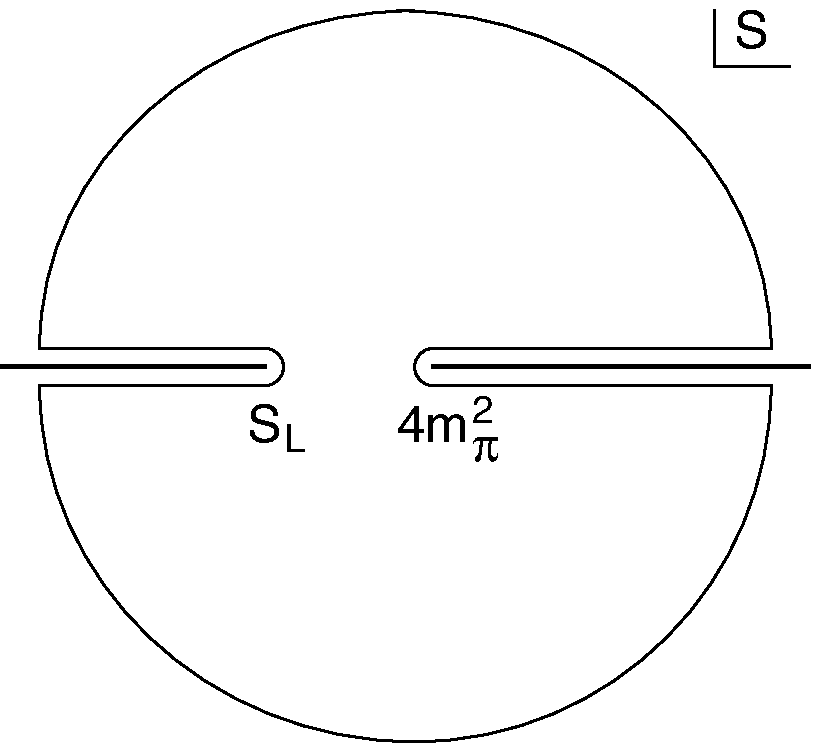
\includegraphics[width=4cm]{bk-fig1}}
\caption{Sample figure caption.}
\label{fig1.1}
\end{figure}
\end{verbatim}
\begin{figure}[h]
\centerline{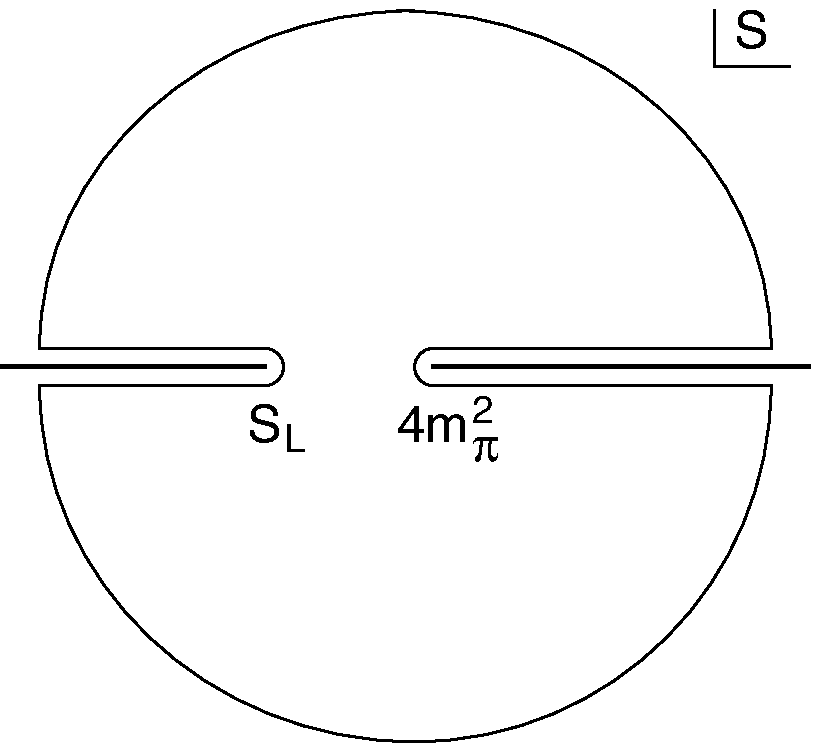
\includegraphics[width=4cm]{bk-fig1}}
\caption{Sample figure caption.}
\label{fig1.1}
\end{figure}

Adjust the scaling of the figure until it is correctly
positioned, and remove the declarations of the lines and any
anomalous spacing.

Here is an example of two figures appearing side-by-side:
\begin{verbatim}
\begin{figure}[ht]
\sidebyside
{
    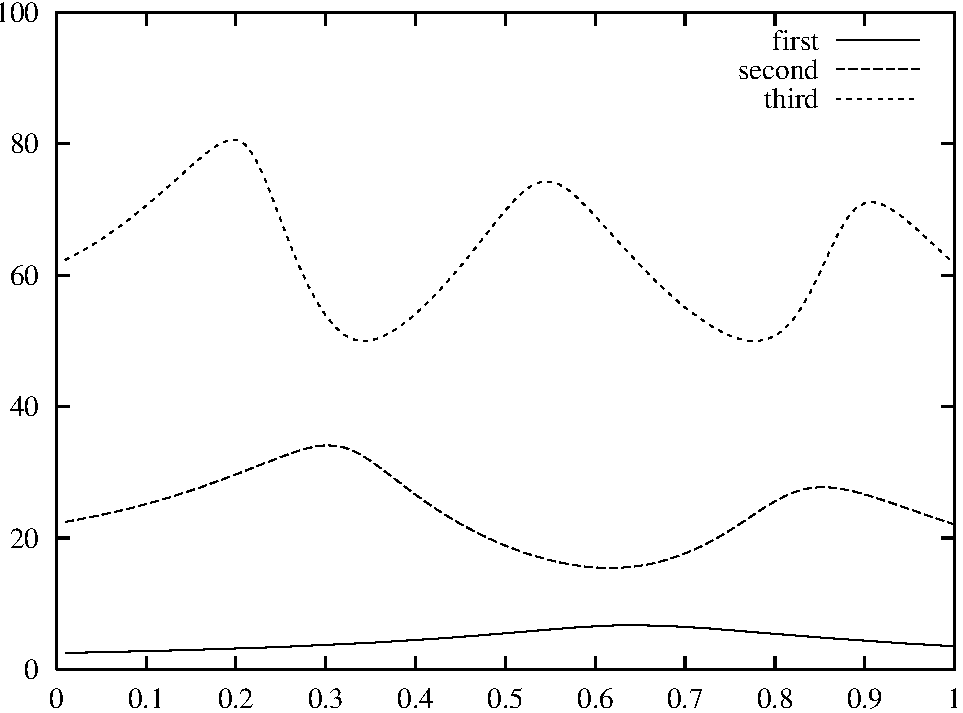
\includegraphics[width=2in]{bk-fig2}
    \caption{Figure caption for left-side figure.}
    \label{fig1.2}
}{
    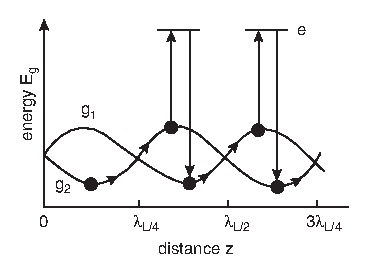
\includegraphics[width=2in]{bk-fig3}
    \caption{Figure caption for right-side figure.}
    \label{fig1.3}
}
\end{figure}
\end{verbatim}

\begin{figure}[ht]
\sidebyside
{
    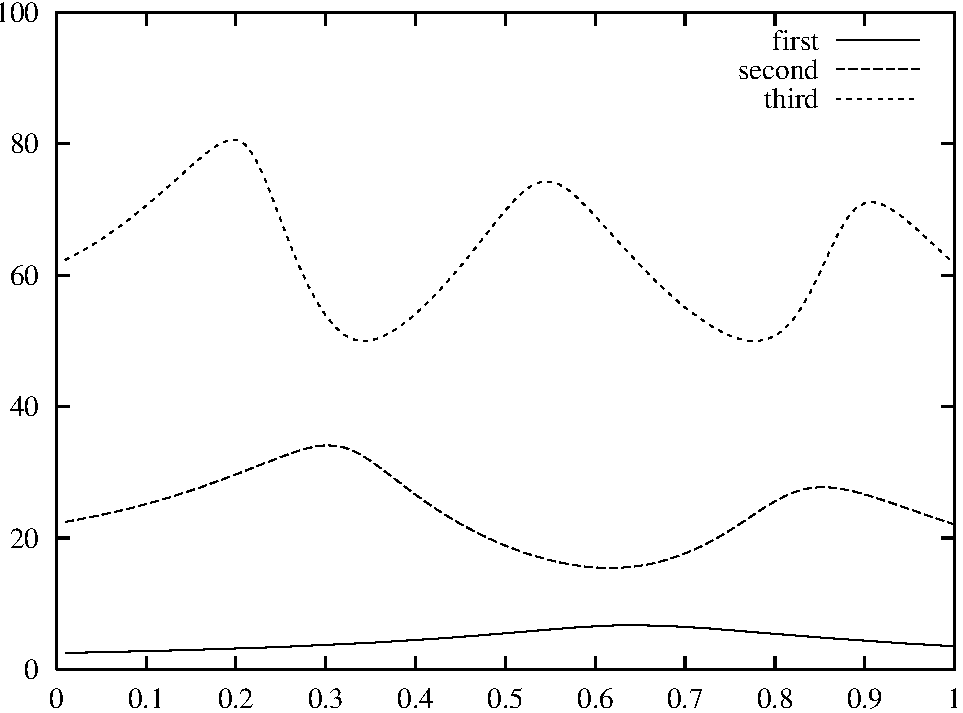
\includegraphics[width=2in]{bk-fig2}
    \caption{Left-side figure caption.}\label{fig1.2}
}{
    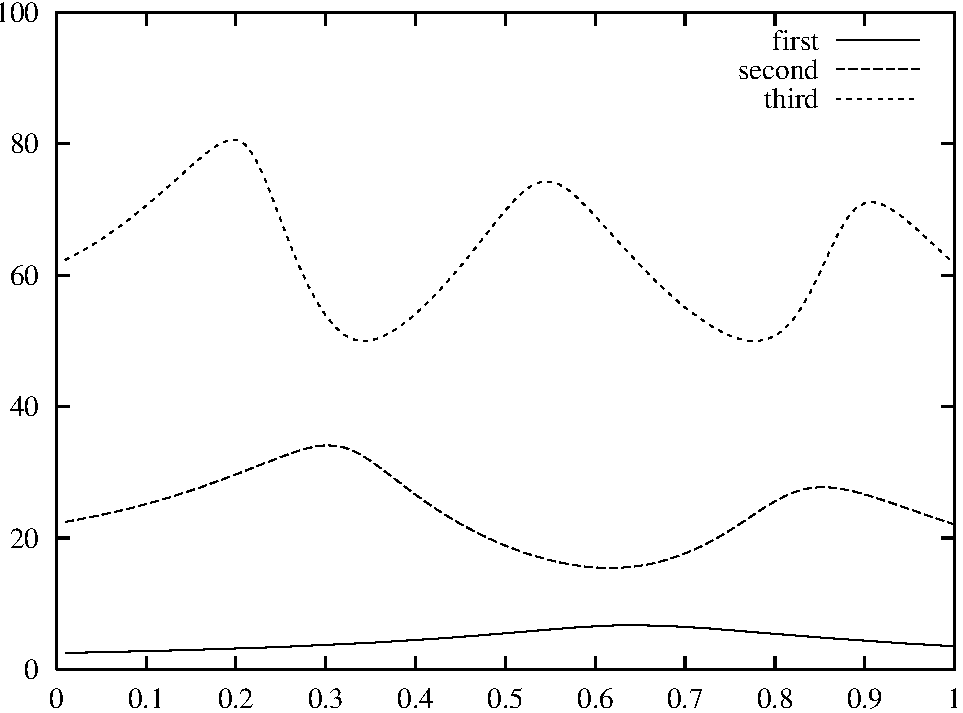
\includegraphics[width=2in]{bk-fig2}
    \caption{Right-side figure caption.}\label{fig1.3}
}
\end{figure}

Here is an example of two figures appearing side-by-side with single caption:

\def\sbs{\hsize=.45\textwidth\parindent=0pt\centering}
\long\def\sidebyside#1#2{\figurecaptionfont
\hbox to\textwidth{\vtop{\sbs#1\vskip1sp}\hfill\vtop{\sbs#2}}}

\begin{verbatim}
\begin{figure}[ht]
\sidebyside
{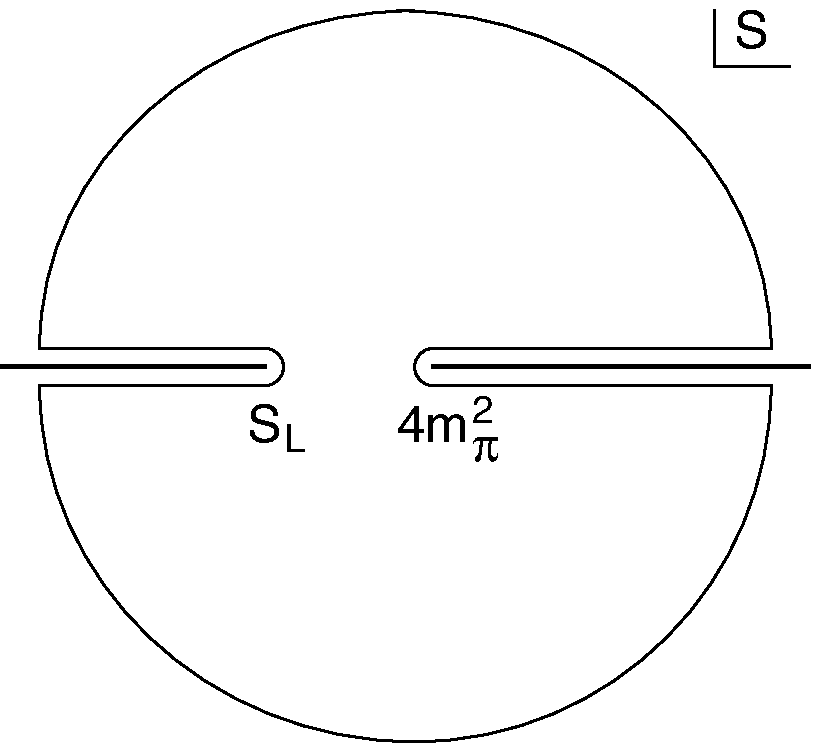
\includegraphics[width=1.8in]{bk-fig1}\\(a)}
{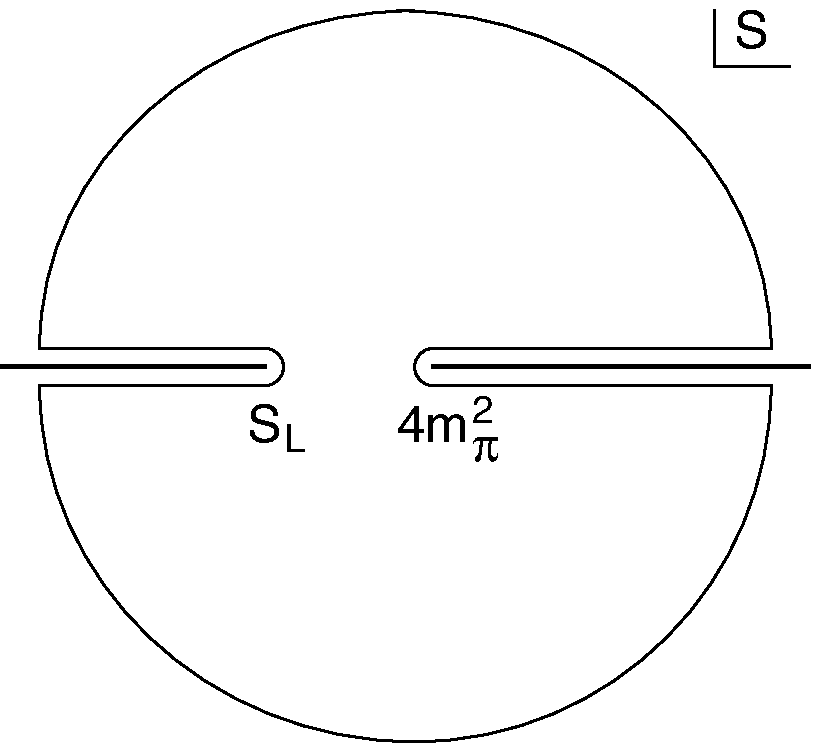
\includegraphics[width=1.8in]{bk-fig1}\\(b)}
\caption{Two figures side-by-side.
         (a) Figure caption for left-side figure.
         (b) Figure caption for right-side figure.}
\label{fig1.4}
\end{figure}
\end{verbatim}

\begin{figure}[ht]
\sidebyside
{
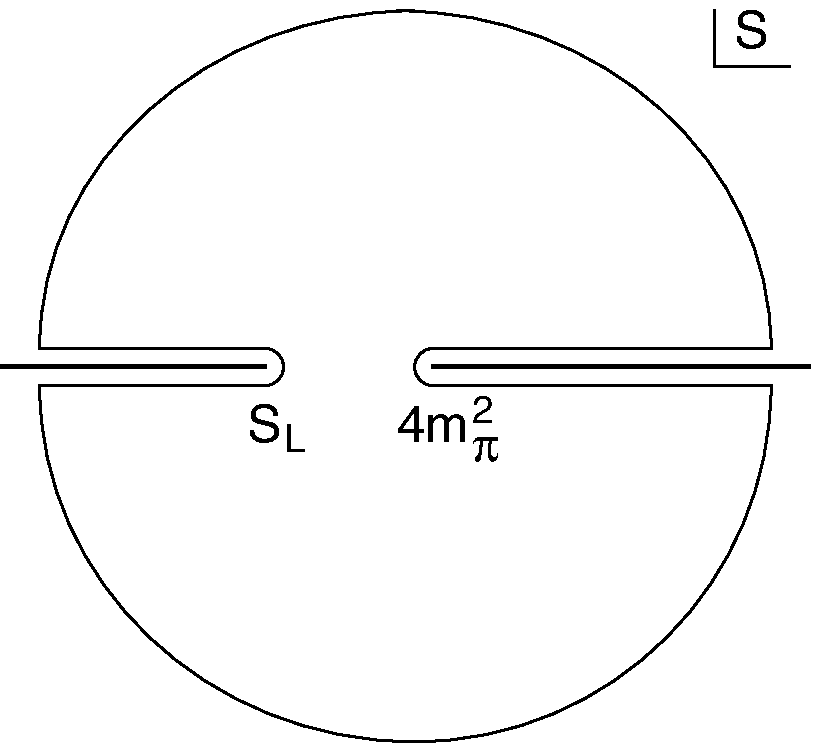
\includegraphics[width=1.8in]{bk-fig1}\\(a)
}
{
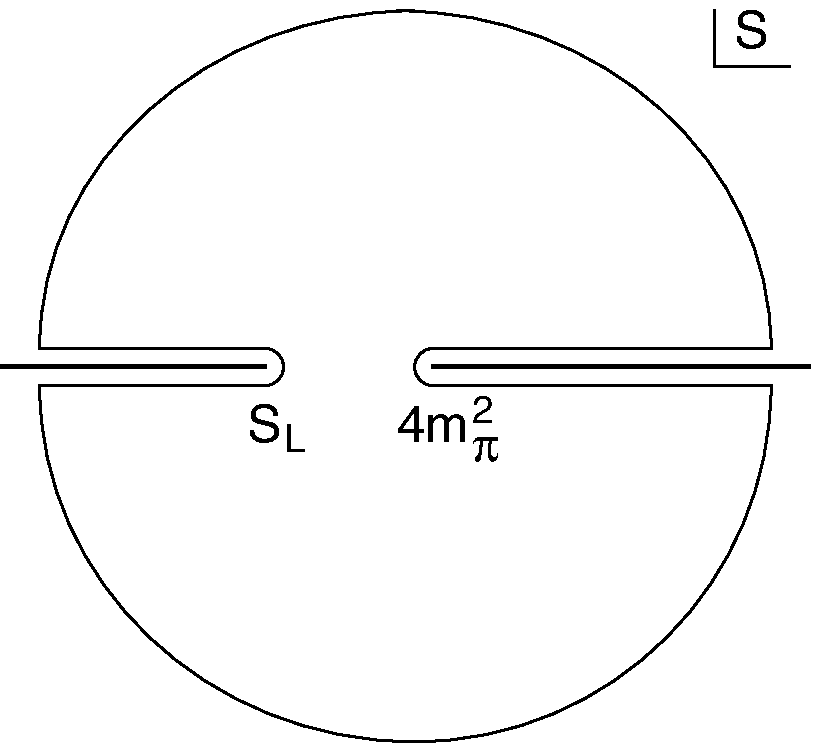
\includegraphics[width=1.8in]{bk-fig1}\\(b)
}
\caption{Two figures side-by-side.
         (a) Figure caption for left-side figure.
         (b) Figure caption for right-side figure.}
\label{fig1.4}
\end{figure}

Side-by-side figures Fig.~\ref{fig1.4}(a) and \fref{fig1.4}(b) are
referred with \verb|Fig.~\ref{fig1.4}(a)| and
\verb|\fref{fig1.4}(b)| commands.

If instead you wish to use some other method, then it is very
important to leave the right amount of vertical space in the figure
declaration to accommodate your figure.

The preferred graphics formats are tiff and Encapsulated PostScript
(eps), for any type of image. The WSPC \TeX\ installation requires
eps, but we can easily convert tiff to eps. Many other formats,
e.g.~pict (Macintosh), wmf (Windows) and various proprietary
formats, are not suitable. Even if we can read such files, there is
no guarantee that they will look the same on our systems as on
yours.

\begin{sidewaysfigure}\index{floats!figures!landscape}
\begin{center}
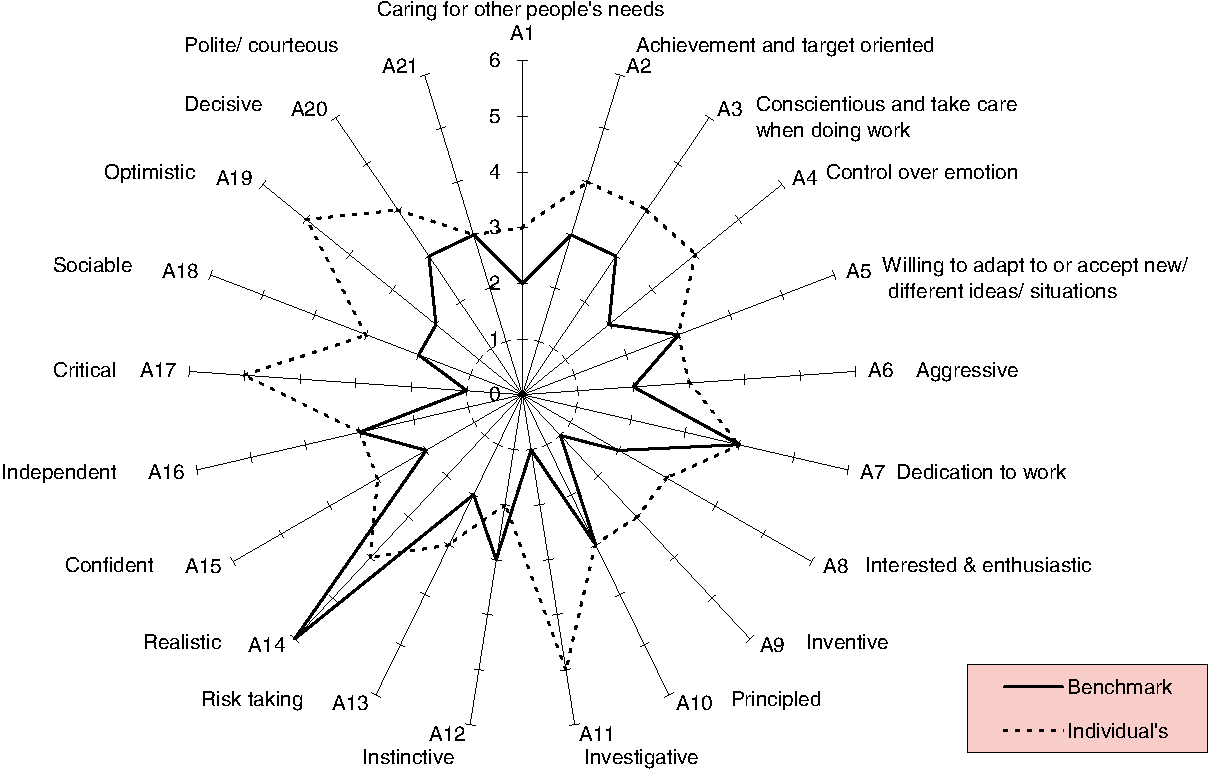
\includegraphics[height=4in]{bk-fig5}
\end{center}
\caption{Landscape figure.}
\label{fig1.5}
\end{sidewaysfigure}

\def\p{\phantom{$-$}}
\def\pc{\phantom{,}}
\def\p0{\phantom{0}}
\begin{sidewaystable}
\tbl{Landscape table.}
{\begin{tabular}{@{}ccccccccccc@{}}
\toprule\\[-6pt]
$f_0$ &$\lambda_0$ &$\alpha_0$
&\multicolumn{8}{c}{Positive roots ($X_0$)}\\[3pt]
\hline\\[-6pt]
&& &4D &5D &6D &7D &8D &10D &12D &16D\\[3.5pt]
\hline\\[-6pt]
\phantom{1}$-0.033$ &0.034 &\phantom{0}0.1\phantom{.01} &6.75507\p0
&4.32936\p0 &3.15991\p0 &2.44524\p0
&1.92883\p0 &0.669541 &--- &---\\[3.5pt]
&&&1.14476\pc\p0 &1.16321\pc\p0 &1.1879\pc\phantom{00}
&1.22434\pc\p0 &1.29065\pc\p0
&0.415056\pc\\[3.5pt]
\phantom{1}$-0.1$\phantom{33} &0.333 &\phantom{0}0.2\phantom{.01}
&3.15662\p0 &1.72737\p0 &--- &--- &--- &--- &--- &---\\[3.5pt]
&&&1.24003\pc\p0 &1.48602\pc\p0\\[3.5pt]
\phantom{1}$-0.301$ &0.302 &0.001
&2.07773\p0 &--- &--- &--- &--- &--- &--- &---\\[3.5pt]
&&&1.65625\pc\p0\\[3.5pt]
\phantom{1}$-0.5$\phantom{01} &0.51\phantom{2} &\phantom{0}0.001
&--- &--- &--- &--- &--- &--- &--- &---\\[3.5pt]
$\phantom{1-}$0.1\phantom{01} &0.1\phantom{02}
&\phantom{0}2\phantom{.001} &1.667\phantom{000}
&1.1946\phantom{00,}
&--- &--- &--- &--- &--- &---\\[3.5pt]
&&&0.806578\pc &0.858211\pc\\[3.5pt]
$\phantom{1-}$0.1\phantom{01} &0.1\phantom{33} &10\phantom{.001}
&0.463679\pc &0.465426\pc &0.466489\pc &0.466499\pc
&0.464947\pc &0.45438\pc\p0 &0.429651\pc &0.35278\pc\\[3.5pt]
$\phantom{1-}$0.1\phantom{01} &1\phantom{.333}
&\phantom{0}0.2\phantom{01}
&--- &--- &--- &--- &--- &--- &--- &---\\[3.5pt]
$\phantom{1-}$0.1\phantom{01} &5\phantom{.333}
&\phantom{0}5\phantom{.001}
&--- &--- &--- &--- &--- &--- &--- &---\\[3.5pt]
$\phantom{-0}$1\phantom{.033} &0.001 &\phantom{0}2\phantom{.001}
&0.996033 &0.968869 &0.91379\p0 &0.848544&0.783787 &0.669541
&0.577489 &---\\[3.5pt]
&&&0.414324\pc &0.41436\pc\p0 &0.414412\pc &0.414489\pc &0.414605\pc
&0.415056\pc &0.416214\pc\\[3.5pt]
\phantom{10}\phantom{.033} &0.001 &\phantom{0}0.2\phantom{01}
&0.316014 &0.309739 &--- &--- &--- &--- &--- &---\\[3.5pt]
&&&0.275327\pc &0.275856\pc\\[3.5pt]
\phantom{10}\phantom{.033} &0.1\phantom{33}
&\phantom{0}5\phantom{.001} &0.089435\pc &0.089441\pc &0.089435\pc
&0.089409\pc &0.08935\pc\p0
&0.089061\pc &0.088347\pc &0.084352\pc\\[3.5pt]
\phantom{10}\phantom{.033} &1\phantom{.333}
&\phantom{0}3\phantom{.001} &0.128192\pc &0.128966\pc &0.19718\p0
&0.169063 &0.142103
&--- &--- &---\\[3.5pt]
&&&& &0.41436\pc\p0 &0.414412\pc &0.414489\pc\\[3pt]
\Hline
\end{tabular}}\label{tbl1.2}
\end{sidewaystable}

Very large figures and tables should be placed on a page by
themselves. Landscape tables and figures can be typeset with
following environments:

\begin{itemize}\index{floats!tables!landscape}
\item[$\bullet$] \verb|sidewaystable| and
\item[$\bullet$] \verb|sidewaysfigure|.
\end{itemize}

\noindent {\bf Example:}

\begin{verbatim}
\begin{sidewaysfigure}
\begin{center}
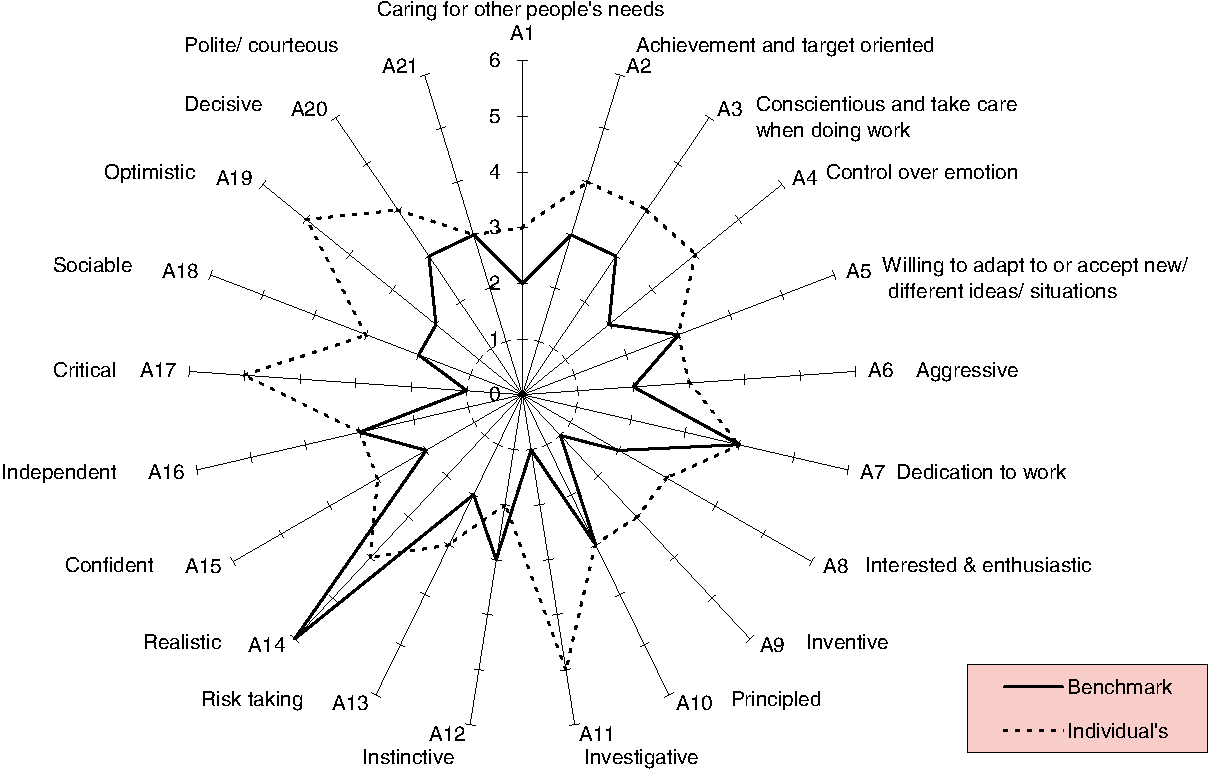
\includegraphics[height=4in]{bk-fig5}
\end{center}
\caption{Sample figure caption.}
\label{fig1.5}
\end{sidewaysfigure}
\end{verbatim}

\section{Proofs}
The WSPC document styles also provide a pre-defined proof
environment for proofs. The proof environment produces the heading
`Proof' with appropriate spacing and punctuation. A `Q.E.D.' symbol,
$\square$, can be appended at the end of a proof with the command
\verb|\qed|., e.g.

\begin{verbatim}
\begin{proof}
This is a test.
\end{proof}
\end{verbatim}

\noindent to produce

\begin{proof}
This is a test.
\end{proof}

If you want to display, `Proof of Lemma', then write

\begin{verbatim}
\begin{proof}[Proof of Lemma]
This is a test.
\end{proof}
\end{verbatim}

\noindent to produce

\begin{proof}[Proof of Lemma]
This is a test.
\end{proof}

\section{Theorems and Definitions}\index{theorems}
The WSPC document styles contain a set of pre-defined
environments for theorems, definitions, proofs, remarks etc., e.g.

All theorem-like objects use individual numbering scheme by default.
To number them in a single sequence, load the class option
\verb|onethmnum| in the preamble., e.g., \verb|\documentclass[onethmnum]{ws-book9x6}|.

\begin{verbatim}
\begin{theorem}
We have $\# H^2 (M \supset N) < \infty$ for an inclusion ...
\end{theorem}
\end{verbatim}

\noindent produces

\begin{theorem}
We have $\# H^2 (M \supset N) < \infty$ for an inclusion $M \supset
N$ of factors of finite index.
\end{theorem}

\begin{verbatim}
\begin{theorem}[Longo, 1998]
For a given $Q$-system...
\[
N = \{x \in N; T x = \gamma (x) T, T x^* = \gamma (x^*) T\}\,,
\]
and $E_\Xi (\cdot) = T^* \gamma (\cdot) T$ gives a conditional
expectation onto $N$.
\end{theorem}
\end{verbatim}

\noindent generates

\begin{theorem}[Longo, 1998]
For a given $Q$-system...
\[
N = \{x \in N; T x = \gamma (x) T, T x^* = \gamma (x^*) T\}\,,
\]
and $E_\Xi (\cdot) = T^* \gamma (\cdot) T$ gives a conditional
expectation onto $N$.
\end{theorem}

The following environments are available by default with \verb|ws-book-thm| package:

\begin{center}
{\tablefont
\begin{tabular}{ll}
\toprule Environment & Heading\\\colrule
\verb|algorithm| & Algorithm\\
\verb|answer| & Answer\\
\verb|assertion| & Assertion\\
\verb|assumption| & Assumption\\
\verb|case| & Case\\
\verb|claim| & Claim\\
\verb|comment| & Comment\\
\verb|condition| & Condition\\
\verb|conjecture| & Conjecture\\
\verb|convention| & Convention\\
\verb|corollary| & Corollary\\
\verb|criterion| & Criterion\\
\verb|definition| & Definition\\
\verb|example| & Example\\
\verb|lemma| & Lemma\\
\verb|notation| & Notation\\
\verb|note| & Note\\
\verb|observation| & Observation\\
\verb|problem| & Problem\\
\verb|proposition| & Proposition\\
\verb|question| & Question\\
\verb|remark| & Remark\\
\verb|solution| & Solution\\
\verb|step| & Step\\
\verb|summary| & Summary\\
\verb|theorem| & Theorem\\\botrule
\end{tabular}}\label{theo}
\end{center}

\LaTeX{} provides \verb|\newtheorem| to create new theorem
environments. To add a new theorem-type environments to a chapter, use

\begin{verbatim}
\newtheorem{example}{Example}[section]

\let\Examplefont\upshape

\def\Exampleheadfont{\bfseries}
\end{verbatim}

(See the \LaTeX{} user manual \cite{lamp94,ams04}.)

\section{Cross-referencing}
Use \verb|\label| and \verb|\ref| for cross-referencing to
equations, figures, tables, sections, subsections, etc., instead of
plain numbers. Every numbered part to which one wants to refer
should be labelled with the instruction \verb|\label|, e.g.

\begin{verbatim}
\begin{equation}
\mu(n, t) = \frac{\sum\limits^\infty_{i=1}1 ...}
\label{eq1.1}
\end{equation}
\end{verbatim}

With the instruction \verb|\ref| one can refer to a numbered part
that has been labelled, e.g. \verb|..., see also Eq. (\ref{eq1.1})|.

\begin{center}{\tablefont
Some useful shortcut commands.
\begin{tabular}{lll}
\toprule
Shortcut & Equivalent & Output \\
command & \TeX\ command\\\colrule
\multicolumn{3}{@{}l}{In the middle of a sentence:}\\
\verb|\eref{eq1.1}|  & Eq.~(\verb|\ref{eq1.1}|) & \eref{eq1.1}\\
\verb|\sref{sec1.1}| & Sec.~\verb|\ref{sec1.1}| & \sref{sec1.1}\\
\verb|\cref{ch1}|  & Chap.~\verb|\ref{ch1}| & \cref{ch1}\\
\verb|\fref{fig1.1}| & Fig.~\verb|\ref{fig1.1}|  & \fref{fig1.1}\\
\verb|\tref{tbl1.1}| & Table~\verb|\ref{tbl1.1}|  & \tref{tbl1.1}\\[3pt]
\multicolumn{2}{@{}l}{At the starting of a sentence:}\\
\verb|\Eref{eq1.1}|  & Equation (\verb|\ref{eq1.1}|) & \Eref{eq1.1}\\
\verb|\Sref{sec1.1}| & Section~\verb|\ref{sec1.1}| & \Sref{sec1.1}\\
\verb|\Cref{ch1}|  & Chapter~\verb|\ref{ch1}| & \Cref{ch1}\\
\verb|\Fref{fig1.1}| & Figure~\verb|\ref{fig1.1}| & \Fref{fig1.1}\\
\verb|\Tref{tbl1.1}| & Table~\verb|\ref{tbl1.1}| & \Tref{tbl1.1}\\\botrule
\end{tabular}}
\end{center}

\begin{itemize}
\item[$\bullet$] The \verb|\label| instruction should be typed
immediately after (or one line below), but not inside the argument of
a number-generating instruction such as \verb|\section| or \verb|\caption|, e.g.\\
\verb|\caption{ ... caption ... }\label{fig1.1}|
\item[$\bullet$] but for chapters, label should be placed as\\
    \verb|\chapter{Chapter Title\label{ch1}}|.
\item[$\bullet$] labels should not be repeated.
\end{itemize}

\section{Citations}\index{citation}

World Scientific's preferred style for books is the Harvard (author-date) system,
unless the text is very heavily referenced in which case the
Vancouver (numbered) system may be more appropriate.

\begin{center}
\tablefont
\begin{tabular}{@{}ll@{}}\toprule
System & Package\\\colrule
 Harvard (author-date) & \verb|\usepackage{ws-book-har}|\\
 Vancouver (numbered)\\
 \quad$\bullet$ Bracketed [1] & \verb|\usepackage{ws-book-van}|\\
 \quad$\bullet$ Superscript$^1$ & \verb|\usepackage[super]{ws-book-van}|\\\botrule
\end{tabular}
\end{center}

\subsection{Harvard Style}\index{citation!author-date}

Use \verb|\bibitem| to produce the bibliography.  Citations in the
text use the labels defined in the \verb|bibitem| declaration, for example,
the first paper by \cite{jarl88} is cited using the command
\verb|\cite{jarl88}|. The bibitem labels should not be repeated.

Basic citation commands available with the \verb|ws-book-har| package:

\

\noindent{\tablefont
\begin{tabular}{l@{\quad$\Rightarrow$\quad}l}
\verb|\citeauthor{weis94}|  & \citeauthor{weis94}\\
\verb|\citeyear{weis94}|  & \citeyear{weis94}\\
\verb|\cite{weis94}|  & \cite{weis94}\\
\verb|\cite[Chap. 1]{weis94}|  & \cite[Chap. 1]{weis94}\\
\verb|\citet{weis94}| & \citet{weis94}\\
\verb|\citep{weis94}| & \citep{weis94}\\
\verb|\citep[Chap. 1]{weis94}| & \citep[Chap. 1]{weis94}\\
\verb|\citep[see][]{weis94}| & \citep[see][]{weis94}\\
\verb|\citep[see][Chap. 1]{weis94}| & \citep[see][Chap. 1]{weis94}\\
\verb|\cite{best03,chur90}| & \cite{best03,chur90}\\
\verb|\citet{best03,chur90}| & \citet{best03,chur90}\\
\verb|\citep{best03,chur90}| & \citep{best03,chur90}\\
\end{tabular}}

\begin{itemize}
\item[$\bullet$] For a single author, use `\citet{weis94} ...' or
`... \cite{weis94}'
\item[$\bullet$] For multiple citations, do not use \verb|\cite{chur90}\cite{weis94}|, but use
\verb|\cite{chur90,weis94}| instead.
\item[$\bullet$] If there are two authors, use \cite{chur90} or \citep{chur90}
\item[$\bullet$] Add a, b, c, etc.~to distinguish between two or
more references with the same author name and year (e.g., Roitt
1999a,b)
\end{itemize}

\subsection{Vancouver Style}\index{citation!numbered}

Reference citations in the text are to be numbered consecutively in
Arabic numerals, in the order of first appearance. The numbered citations
can appear in two ways:

\begin{enumerate}
\item[(i)] bracketed
\item[(ii)] superscript
\end{enumerate}

\subsubsection{Bracketed}\index{citation!numbered!bracketed}
References cited in the text are within square brackets, e.g.,

\begin{enumerate}
\item[(1)] \verb|``One can deduce from Ref.~\cite{benh93} that...''|\\
            ``One can deduce from Ref.~[3] that...''
\smallskip
\item[(2)] \verb|``See Refs.~\cite{ams04,bake72,benh93,brow88} and|\\
      \verb|\cite{davi93} for more details.''|\\
      ``See Refs.~[1--3, 5] and [7] for more details.''
\end{enumerate}

\subsubsection{Superscript}\index{citation!numbered!superscript}

References cited in the text appear as superscripts, e.g.,

\begin{enumerate}
\item[(1)] \verb|``...in the statement.\cite{ams04}''|\\
            ``...in the statement.$^1$''
\smallskip
\item[(2)] \verb|``...have proven\cite{bake72} that this equation...''|\\
            ``...have proven$^2$ that this equation...''
\end{enumerate}

When the reference forms part of the sentence, it should appear with
``Reference'' or ``Ref.'', e.g.,

\begin{enumerate}
\item[(1)] \verb|``One can deduce from Ref.~\refcite{benh93} that...''|\\
      ``One can deduce from Ref.~3 that...''
\smallskip
\item[(2)] \verb|``See Refs.~\refcite{ams04}--\refcite{benh93},|
      \verb|\refcite{brow88} and \refcite{davi93} for more details.''|\\
     ``See Refs.~1--3, 5 and 7 for more details.''
\end{enumerate}

\section{Footnote}\index{footnote}
Footnotes are denoted by Arabic number superscript in the text, e.g.,

\

\noindent {\bf Usage:}
\begin{verbatim}
... total.\footnote{Sample footnote text.}
\end{verbatim}

\noindent {\bf Output:}

\noindent ... in total.\footnote{Sample footnote text.}

\section{Running Heads}\index{running head}
The WSPC prefers ``Book Title'' as even page header and ``Chapter Title'' as odd page header.
However, authors can pick their required style by switching the class options while loading the \verb|ws-book9x6| document class in the preamble.

\begin{table}[h]
\centerline
{\tablefont\begin{tabular}{@{}lll@{}}\toprule
Class options&Even page& Odd page\\\colrule
{\tt$\backslash$documentclass[acrhead]}\{{\tt{ws-book9x6}}\}$^{\textrm a}$ & Author Name(s) & Chapter Title\\
{\tt$\backslash$documentclass[csrhead]}\{{\tt{ws-book9x6}}\} & Chapter Title & Section Title\\
{\tt$\backslash$documentclass}\{{\tt{ws-book9x6}}\} & Book Title & Chapter Title\\\botrule
\end{tabular}}
\begin{tabnote}
$^{\textrm a}$Author names are included with \verb|\author{A. Author}| in multi-authored books.
\end{tabnote}
\label{tbl1.3}
\end{table}

\section{Miscellaneous}
\subsection{Quote}\index{quote}
Here is an example for the \verb|quote| environment.

\begin{quote}
This is an example for the \verb|quote| environment. Quote text is
indented by 1pc on the left and right sides. The point size for the
quote text is 9/11pt.
\end{quote}

\section{Acknowledgments and Appendices}\index{acknowledgments}
Acknowledgments to funding bodies, etc. may be placed in a separate
section at the end of the text, before the appendices. This should not
be numbered, so use \verb|\section*{Acknowledgements}|.

\section{Appendices}\index{appendix}
Appendices should be used only when absolutely necessary. They
should come before the bibliography. Appendix A of this
document has more details on appendices.

\section{Bibliography}\index{bibliography}

\subsection[BiBTeX users]{\btex\ users}

\btex\index{\btex} users should use our bibliography style file
\verb|ws-book-har.bst| for (author-date) references or
\verb|ws-book-van.bst| for (numbered) references. \Cref{ch2} of this
document has more on \btex.

\subsection[Non-BiBTeX users]{Non-\btex\ users}
Non-\btex\ users can follow the reference pattern as shown below.

Here is some sample coding for author-date\index{bibliography!author-date} references.

\begin{verbatim}
\begin{thebibliography}{9}
\bibitem[{\AmS(2004)}]{ams04}
\AmS (2004). \emph{\AmS-\LaTeX{} Version 2 User's Guide}
  (American Mathematical Society, Providence),
  \url{http://www.ams.org/tex/amslatex.html}.

\bibitem[{Baker and Carter(1972)}]{bake72}
Baker, D.~W. and Carter, N.~L. (1972). \emph{Seismic Velocity
  Anisotropy Calculated for Ultramafic Minerals and
  Aggregates}, \emph{Geophys. Mono.}, Vol.~16 (Am. Geophys.
  Union), pp. 157--166.

\bibitem[{Benhamou and Colmerauer(1993)}]{benh93}
Benhamou, F. and Colmerauer, A. (eds.) (1993). \emph{Constraint
  Logic Programming, Selected Research} (MIT Press).
\bibitem[{Bestbury(2003)}]{best03}
Bestbury, B.~W. (2003). $R$-matrices and the magic square,
  \emph{J. Phys. A} \textbf{36}, 7, pp. 1947--1959.
\end{thebibliography}
\end{verbatim}

Here is some sample coding for numbered\index{bibliography!numbered} references.

\begin{verbatim}
\begin{thebibliography}{9}
\bibitem{ams04}
\AmS (2004). \emph{\AmS-\LaTeX{} Version 2 User's Guide}
  (American Mathematical Society, Providence),
  \url{http://www.ams.org/tex/amslatex.html}.

\bibitem{bake72}
Baker, D.~W. and Carter, N.~L. (1972). \emph{Seismic Velocity
  Anisotropy Calculated for Ultramafic Minerals and
  Aggregates}, \emph{Geophys. Mono.}, Vol.~16 (Am. Geophys.
  Union), pp. 157--166.

\bibitem{benh93}
Benhamou, F. and Colmerauer, A. (eds.) (1993). \emph{Constraint
  Logic Programming, Selected Research} (MIT Press).

\bibitem{best03}
Bestbury, B.~W. (2003). $R$-matrices and the magic square,
  \emph{J. Phys. A} \textbf{36}, 7, pp. 1947--1959.
\end{thebibliography}
\end{verbatim}

The only difference between the codings of author-date references
and numbered references is the argument of \verb|\bibitem|.

\begin{center}\tablefont
\begin{tabular}{@{}ll@{}}\toprule
Author-date & Numbered\\\colrule
\verb|\bibitem[{\AmS(2004)}]{ams04}|... &\verb|\bibitem{ams04}|...\\
\verb|\bibitem[{Baker and Carter(1972)}]{bake72}|... &\verb|\bibitem{bake72}|...\\
\verb|\bibitem[{Bestbury(2003)}]{best03}|... &\verb|\bibitem{best03}|...\\
\botrule
\end{tabular}
\end{center}

\section{Index}\index{index}
The index should be printed at the end of the book. \Cref{ch3} has more
on indexing.
